
\part[Subalgoritmos]
{Funções}


\chapter[Subalgoritmos]
{Funções}



\section*{Resumo}

Uma função é um conjunto de instruções que, ao final da função, executa uma tarefa. Todo programa C possui pelo menos uma função, a \emph{main}.

%\begin{chapreferences}{1.}
%\bibliography{playcb}
%\bibliographystyle{plain}
%\nocite{cbook}
%\nocite{sb6}
%\nocite{glfw}
%\nocite{cppbook}

%\end{chapreferences}

% \begin{chapreferences}{1}

% \bibitem{sb6}
% {\em OpenGL SuperBible}.
% \newblock Pearson Education Inc, 6 edition, 2014.

% \bibitem{glfw}
% Marcus Geelnard and Camilla Berglund.
% \newblock {\em GLFW - Reference guide}, 2010.
% \newblock API version 2.7.

% \bibitem{cbook}
% Brian~W. Kernighan and Dennis~M. Ritchie.
% \newblock {\em The C Programming Language}.
% \newblock 1989.

% \bibitem{cppbook}
% Stanley~B. Lippman, Josés Lajoile, and Barbara Moo.
% \newblock {\em C++ Primer}.
% \newblock 2013.
% \end{chapreferences}

\section*{Pré-requisitos}

As práticas deste capítulo exigem que sejam utilizadas as funções
\begin{itemize}
  \item 
    \begin{lstlisting}[language=C++]
    void LimpaDesenho()
    \end{lstlisting}

  \item 
    \begin{lstlisting}[language=C++]
    void ApagaGrupo(int index)
    \end{lstlisting}
 
 
\end{itemize}

\section*{Problemas}
\begin{enumerate}
\item
  Crie dois retângulos e posicione-os aleatoriamente em $x$. Coloque uma circunferência no topo do primeiro retângulo e receba do usuário dois valores: ângulo e velocidade. Dado estes valores, calcule e exiba a trajetória balística da circunferência sendo lançada para o outro retângulo. Exiba mensagem caso o usuário consiga acertar o prédio ou não e, em seguida, caso o usuário deseje jogar novamente, sorteie novas posições para os retângulos e execute novamente o procedimento de pedir valores do usuário e exibir a trajetória balística.

  \begin{figure}[ht]
    \centerline{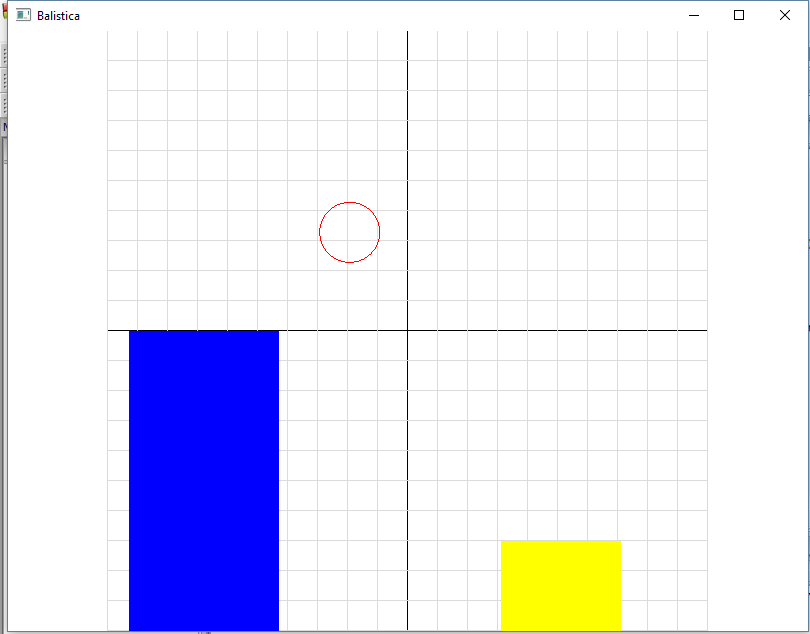
\includegraphics[width=.5\textwidth]{img/cap3_ex12.png}}
    \caption{Lançador Balístico}
    \label{fig:cap03_ex2}
  \end{figure}

  \label{ex:cap03_ex1}

  \item
  Baseado no exercício \ref{ex:cap03_ex1}, faça o Wolverine ser lançado de um prédio, dado um ângulo e uma velocidade inicial, com o objetivo de atacar o Magneto. Se não atingir o Magneto, os dois inimigos se encaram. Se atingir o Magneto, faça o Magneto contra-atacar o Wolverine, lançando o mutante em uma trajetória retilínia na direção contrária ao ataque.

   \begin{figure*}[!htp]
    \centering
    \begin{subfigure}[t]{0.3\textwidth}
        \centerline{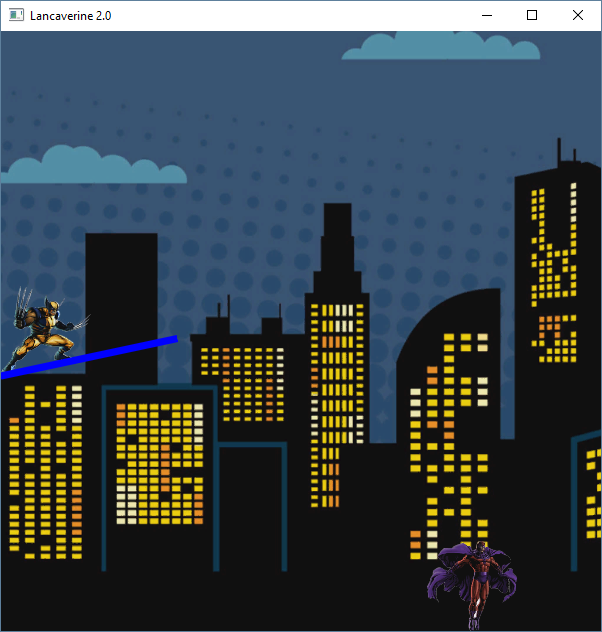
\includegraphics[width=.9\textwidth]{img/cap3_ex27}}
        \caption{Determinação do ângulo}
        \label{fig:cap03_ex27a}
    \end{subfigure}
    \hfill
    \begin{subfigure}[t]{0.3\textwidth}
        \centerline{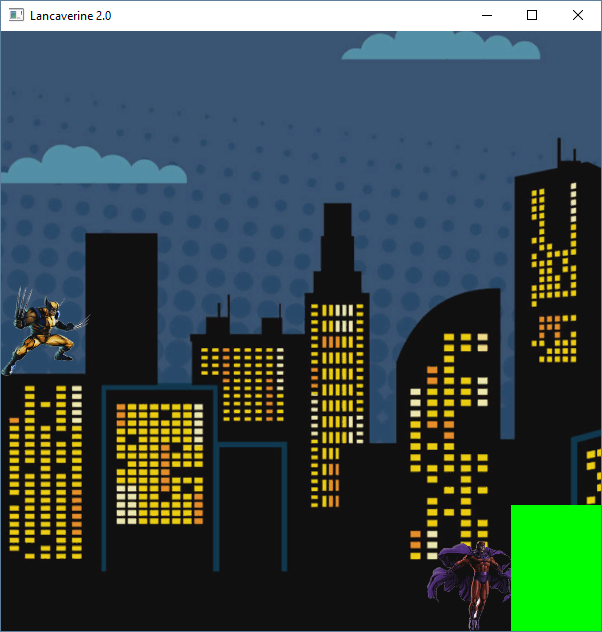
\includegraphics[width=.9\textwidth]{img/cap3_ex27b}}
        \caption{Determinação da velocidade inicial}
        \label{fig:cap03_ex27b}
    \end{subfigure}
    \hfill
    \begin{subfigure}[t]{0.3\textwidth}
        \centerline{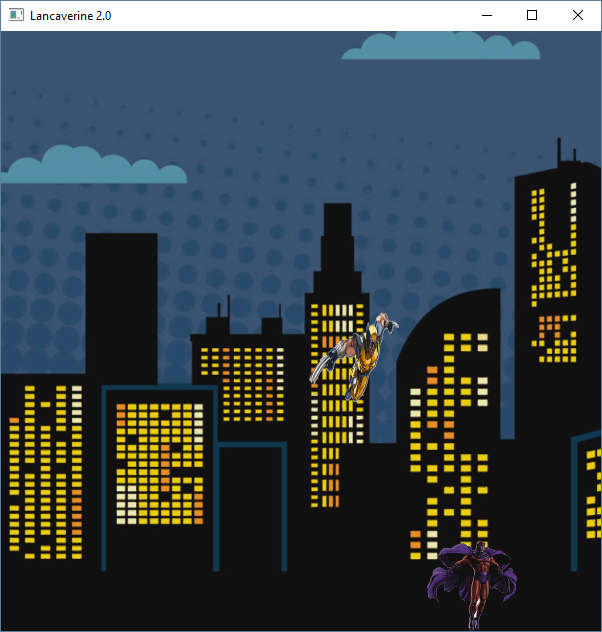
\includegraphics[width=.9\textwidth]{img/cap3_ex27c}}
        \caption{Wolverine sendo lançado}
        \label{fig:cap03_ex27c}
    \end{subfigure}
    \hfill
    \begin{subfigure}[t]{0.3\textwidth}
        \centerline{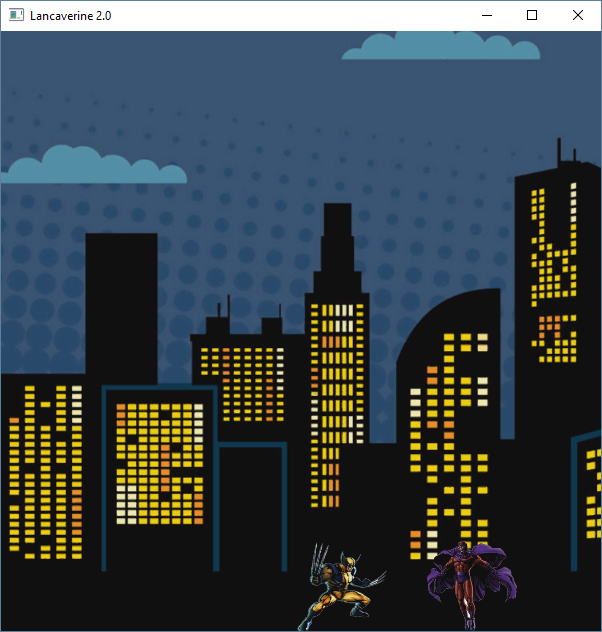
\includegraphics[width=.9\textwidth]{img/cap3_ex27d}}
        \caption{Wolverine e Magneto se encarando}
        \label{fig:cap03_ex27d}
    \end{subfigure}
    ~
    \begin{subfigure}[t]{0.3\textwidth}
        \centerline{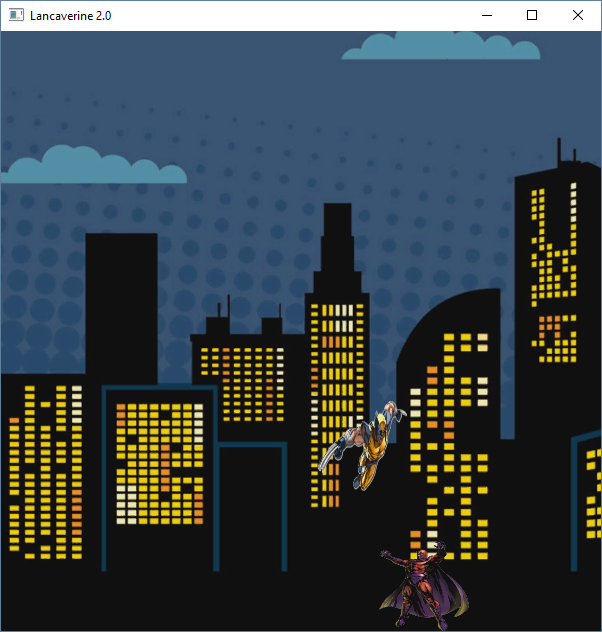
\includegraphics[width=.9\textwidth]{img/cap3_ex27e}}
        \caption{Wolverine sendo lançado pelo Magneto}
        \label{fig:cap03_ex27e}
    \end{subfigure}

  \end{figure*}

  \label{ex:cap03_ex27} 
  
  \newpage
\item
  Crie o jogo Snake com as seguintes configurações
  \begin{itemize}
  \item
    A cabeça não pode estar na mesma posição que o corpo
  \item
    A cabeça não pode estar na mesma posição que a parede
  \end{itemize}
  \emph{SUGESTÃO: Utilize a lógica do exercício \ref{ex:cap02_ex1} }

  \label{ex:cap03_ex2}

  \begin{figure}[H]
    \centerline{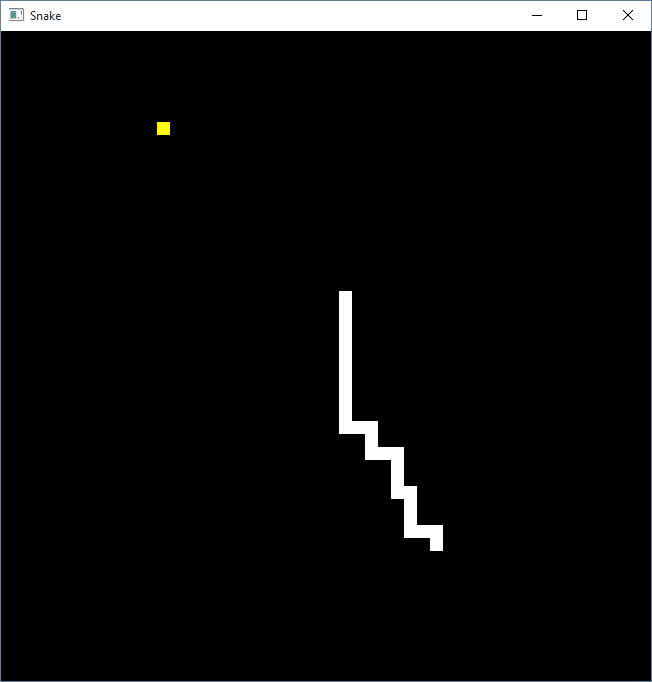
\includegraphics[width=.5\textwidth]{img/cap3_ex10.png}}
    \caption{Jogo Snake}
    \label{fig:cap03_ex2}
  \end{figure}

\end{enumerate}

\section*{Soluções}

\subsection*{Exercício \ref{ex:cap03_ex1} }

Esta prática ilustra como a função \emph{LimpaDesenho} é usada para poder redesenhar outras cenas.
\lstinputlisting[caption=Código fonte do lançador balístico, style=customc, label=lst:cap3_ex1]{src/ex12_balistica.cpp}

\begin{lstlisting}[label={func:LimpaDesenho},language=C++]
void LimpaDesenho() 
\end{lstlisting}
A função \emph{LimpaDesenho}, na linha \ref{line:LimpaDesenho}, destrói todas as geometrias e retorna toda a \emph{playAPC} para o estado padrão, com exceção dos limites do plano cartesiano.

\subsection*{Exercício \ref{ex:cap03_ex27} }

Esta prática exercita o conceito de animação, assim como o exercício \ref{ex:cap01_ex25}. Porém, ela também ilustra como utilizar o conceitos de grupos na playAPC de forma mais eficiente, liberando espaço na memória quando um grupo não é mais utilizado, como o grupo \emph{lancar}, na Listagem \ref{lst:cap3_ex27}.
\lstinputlisting[caption=Código fonte do Lançaverine, style=customc, label=lst:cap3_ex27]{src/ex28_lancaverine.cpp}

\begin{lstlisting}[label={func:ApagaGrupo},language=C++]
void ApagaGrupo(int index)
\end{lstlisting}
A função \emph{ApagaGrupo}, na linha \ref{line:ApagaGrupo}, destrói todas as geometrias de um determinado grupo. Seu argumento é o índice do grupo, retornado pela função \emph{CriaGrupo}


\subsection*{Exercício \ref{ex:cap03_ex2} }

Esta prática ilustra como a função \emph{ApertaTecla} e \emph{MudaLimitesJanela} podem ser utilizadas: a primeira para lidar com input de teclado \footnote{\url{http://playapc.zaghetto.com/funcoes/extras/input/tecla-pressionada}} e a segunda para ajustar o plano onde as geometrias serão desenhadas.
\lstinputlisting[caption=Código fonte de Snake, style=customc, label=lst:cap3_ex1]{src/ex10_snake.cpp}
